\section{Evaluation}
\label{sec:eval}

We conducted several user studies to evaluate ESTHETE, which is a system composed of a data structural graphical representation of news articles with a timeline-based visualisation.
\begin{figure*}[ht]
\caption{A screenshot of our tool visualizing Rape-related cases from India in 2012}
\center{
  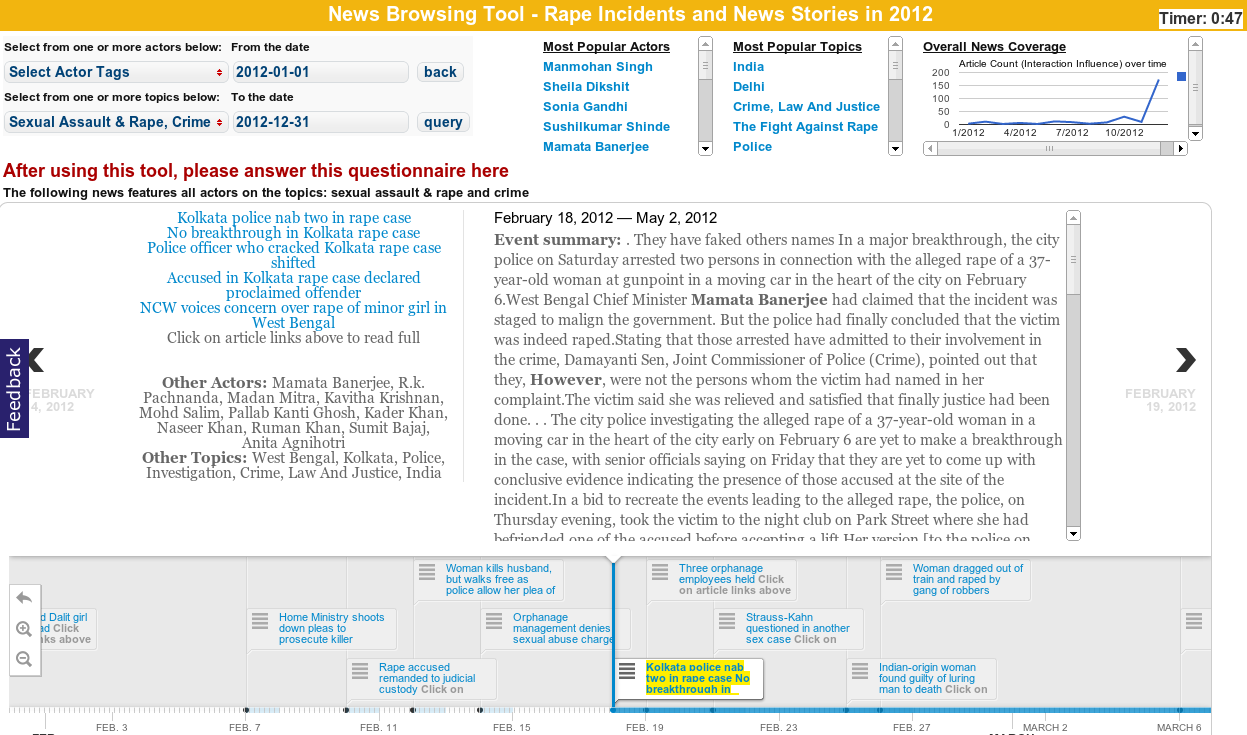
\includegraphics[scale=0.3]{figures/complete.png}
}
\label{fig:complete-tool-screenshot}
\end{figure*}
 %%MR: I have talked specifically about presentation here. Make sure that this has been described somewhere in the text previously. 

\begin{itemize}
	
	\item {\bf Usability and Effectiveness:} For our system to be useful, not only does it have to be easy to use, but also help users understand the big picture of the news story they are interested in. Our experiments in \ref{subsec:usability} evaluates these aspects.
	
	\item {\bf Precision:} A story presented on the timeline has several different aspects associated with it.  A user can filter out the relevant aspects by selecting or deselecting topics and entities identified by the system. The key question we wanted to answer was to find out how effective these filters are in presenting relevant results. Note that the filtering is not a simple keyword filter, but requires that sufficient surrounding context is also retained.
	
	\item {\bf News graphs as a framework:} Finally, our third experiment establishes the usefulness of representing news articles as a graph. We compare our news graph framework to two other baselines -- the articles themselves, and a clustering of articles using k-means clustering.
	
\end{itemize}


\subsection{Setup}
Our news corpus consists of articles published by ``The Hindu'', a popular Indian newspaper. We choose three groups of articles corresponding to ``rape'', ``corruption'' and ``petrol price''. We fired each of these keywords into the website's search form and downloaded all articles that were returned. Therefore, we had three article groups corresponding to the three keywords. The total no. of articles is 10,121, published between 2010-2013. Each group had specific \emph{subsets} of articles corresponding to recent stories in the news. The first group of articles contained, in addition to articles about rape cases in various parts of India and abroad, articles about a gang-rape of a woman on a bus, which led to several weeks of protests in Delhi. Similarly, the second group of articles contained a ``sub-story'' about a very high-profile anti-corruption protests in Delhi, which then morphed into a political story about accusations of corruption against the son-in-law (Robert Vadra) of a powerful politician. The third group of articles contained a sub-story about petrol prices in the year 2012 which lead to political unrest. %%MR: I am not very familiar with this story, please check.

Each article group was then organised as a news graph using the techniques explained in Section \ref{sec:graph-desc}  %we need to mention this 
and the following three sub stories (described in the previous paragraph), were used for experimentation i) the gang-rape incident in Delhi (S1), ii) corruption stories related to Robert Vadra (S2), and, iii) petrol price (S3).

The three user studies made use of the following setup: an article group, in its entirety was presented to the user on our interface. The users were then allowed to interact with the system using whatever filters they felt would be useful. The focus of each set of experiments (described below) were the three sub stories.

%Each of the experiments made use of different kinds of users. For the first experiment of evaluating the precision of our system, we made use of people who had intimate knowledge of the three stories. For the next two experiments the users ranged from college-going students to expert journalists.

\subsection{Results}

\subsubsection{Usability and Effectiveness}
\label{subsec:usability}
\begin{table}
\begin{center}
\small
%\hline
\begin{tabular}{|p{.75cm}|p{.75cm}|p{.75cm}|p{.75cm}|p{.75cm}|p{.75cm}|p{.75cm}|p{.75cm}|}
\hline
\multirow{2}{*}{{\bf Story}} & \multirow{2}{*}{{\bf No. of users}} & \multicolumn{2}{c}{{\bf Ease of use}} & \multicolumn{2}{c}{{\bf New Information}} & \multicolumn{2}{c}{{\bf Big Picture}}\\ \cline{3-8}
& & ESTHETE & Google News & ESTHETE & Google News & ESTHETE & Google News \\
\hline
S1 & 22 & 3.765 & 4.25 & 4.25 & 3.4 & 4.3 & 3.66\\
S2 & 12 & 3.83 & 4.18 & 4.29 & 3.5 & 4.39 & 3.71 \\
S3 & 6 & 3.75 & 4.33 & 4.4 & 3.5 & 4.4 & 3.66\\
\hline
\end{tabular}
\end{center}
\caption{Average ratings for usability}
\label{tab:ease}
\end{table}

\normalsize
In order to evaluate the usability of ESTHETE, we asked 40 users to pick a story of their choice (among S1, S2 and S3) and to study that story by interacting with ESTHETE and Google News, in a random order, for 15 minutes respectively. After the users had interacted with both the systems, we asked users the following questions:

\begin{itemize}
	\item {\bf (Q1) Ease of use:} On a scale of 1 to 5, how would you rate both the systems on their ease of use (with 5 corresponding to ``very easy'')?
	\item {\bf (Q2) New Information:} Given your current knowledge of the story, how would you rate both the systems on their ability to provide new information that you weren't aware of before interacting with the systems? (1 corresponds to ``no new information'', 5 corresponds to ``more than satisfactory'')
	\item {\bf (Q3) Big Picture:} How would you rate both the systems on their ability to aid your understanding of the big picture of the story? (1 corresponds to ``not at all'', 5 corresponds to ``perfectly well'')
\end{itemize}

The results are tabulated in Table \ref{tab:ease}.
Clearly, the users found our system to be more effective than Google News in gaining new information and understanding the bigger picture of the story, in a short time frame. This shows the ability of our system ESTHETE to bring forth and coherently link important nuggets of information. This also exhibits our system's ability to present the user with the necessary context that aided their understanding of the bigger picture of the story. The users also found the system easy to use and navigate.


%%MR: Instead of using ``tool'', use ``system''
Finally, we compared the effectiveness of our system, to help users understand a story in depth, with Google News. We asked 18 users to use either our system or Google News in order to understand any of the three stories listed above. The users had to pick one story of their interest and were allowed to interact with their choosen system for a session lasting 25 minutes. The user's task was to learn as much as they can about their choosen story using a system. Then, once they had completed their interaction with their choosen system (ESTHETE or Google News), they were asked to answer a series of very specific questions related to the story they studied. For example, for the story S2 (Corruption Story), we had questions such as \emph{Do you have information to write a summary of the interactions between Arvind Kejriwal and Robert Vadra?} and \emph{Do you have information to write a summary of the news of Robert Vadra's land dealings in Haryana?}. For these questions, the users had to answer a Yes or a No based on their perception of how easy or difficult they feel it is to answer these questions using the system they just used. The users replied Yes if they felt that they could answer the question using the system they just used and vice versa.

\begin{table}
\small
\begin{center}
\begin{tabular}{|l|p{1.00cm}|p{1.45cm}|p{1.00cm}|p{1.00cm}|p{1.00cm}|}
\hline
%% Rahul: I feel that the column headings of the table are a bit unclear.
{\bf Story} & {\bf No. of responses} & {\bf ESTHETE only} & {\bf Google News only} & {\bf Both} &{\bf None}\\
\hline
S1 & 36 & 23 & 2 & 9 & 2\\
S2 & 12 & 9 & 0 & 2 & 1\\
S3 & 6 & 3 & 0 & 3 & 0 \\
\hline
\end{tabular}
\end{center}
\caption{Effectiveness of ESTHETE}
\label{tab:effectiveness}
\end{table}
\normalsize
The results are tabulated in Table \ref{tab:effectiveness}. The table entries shows for a particular story, the number of responses for which the users responded that they can answer the underlying question using only ESTHETE, only Google News, from both and from none of these systems. The results shows that users found it easier to answer the story-related questions using our system, in comparision to Google News. This clearly demonstrates that our system is more effective than Google News in aiding the users get enough information for answering the story-specific questions. This study brings out the ability of our system to improve the user's understanding of the underlying story.  


\subsubsection{Precision of the system}

\begin{table}
\begin{center}
\small
\begin{tabular}{|c|p{1.25cm}|p{1.25cm}|c|}
\hline
{\bf Story} & {\bf No. of users} & {\bf Avg. no. of filters} & {\bf Precision}\\
\hline
S1 & 10 & 3.4 & 0.89\\
S2 & 10 & 2.5 & 0.92\\
S3 & 8 & 2.1 & 0.88\\
\hline
\end{tabular}
\end{center}
\caption{Precision of articles returned by the system using filters}
\label{tab:prec}
\end{table}

\normalsize

\paragraph*{Description} Users who had intimate knowledge of our three stories were shown the news graph for the entire timeline and allowed to filter these stories using whatever keywords they felt were appropriate from the list of entities and topics extracted by our system. For example, if they filtered on ``Robert Vadra'' (story S2), they would retain articles which not only contained ``Robert Vadra'', but also articles which had a strong connection to him in relation to the corruption allegations against him. The users than judged the relevance of each of these filtered articles on a 2-point scale (either relevant or not relevant). On average, for each story, users used 2-4 filters (that is, they judged the relevance for 2-4 subsets of articles within the larger timeline).

\paragraph*{Results} The results of this experiment are tabulated in Table \ref{tab:prec}. The precision values are in the range 88\%-92\%, indicating that our representation framework is very effective in identifying different contexts.

\eat{
%RG-RM: Some discussion on why the precision values are not 100%

On discussing their assessments with users, we identified two 

%% This first reason about context-adding articles is not quite convincing -- it's like blaming the user.. It might look like users were being very subjective in their assessments -- judging something as relevant only if they did not know about it, rather than ignoring what they know. I have commented both reasons out.
We feel that the precision of our system is not closer to the maximum value of 1 for a variety of reasons. %%MR: Extra discussion.
\begin{itemize}
  \item \textbf {Context-adding articles}: In the hope of adding more context to a user's news browsing experience, we also return articles which are not
  directly related to her input filters, but strongly related to the articles about $P$. However, if the user already has enough context and prior knowledge, 
  such articles become extraneous and are considered irrelevant. For eg., consider a corruption scandal, where a politician $P$ becomes the prime accused
  after a few months of investigation. In such a case, filtering on $P$ also returns articles talking about this case, but not explicitly mentioning $P$.
  For a user with enough prior knowledge of the case, such information is not relevant since she wanted to understand the specific involvement of $P$.
  \item \textbf {Inter-annotator disagreement}: There were cases where two differrent annotators marked the same article as relevant and irrelevant
  respectively on the same task. %%MR: It is no longer ``task'', right? It is the filter. In that case, you should ensure that there are at least 3 annotators and take the majority. Is this the case? If not, I would rather just leave this out.
\end{itemize}
}

\subsubsection{News graphs as a framework}\label{sec:baseline-comparison}
\begin{table}
\begin{center}
\small
\begin{tabular}{|l|p{1cm}|p{1.5cm}|p{1.5cm}|p{1.5cm}|}
\hline
{\bf Story} & {\bf No. of users} & {\bf ESTHETE preferred} & {\bf B1 preferred} & {\bf B2 preferred}\\
\hline
S1 & 7 & 100\% & 0\% & 0\%\\
S2 & 6 & 83\% & 0\% & 17\%\\
S3 & 7 & 100\% & 0\% & 0\%\\
\hline
\end{tabular}
\end{center}
\caption{Comparison of news graphs against baselines B1 and B2} %%MR: Need to change
\label{tab:graph}
\end{table}

\normalsize

\paragraph*{Description} In order to determine whether news graphs compare against other ways of representing news corpora, we designed the following two baselines, both of which also made use of our timeline interface. Our first baseline (B1) simply presents \emph{all} articles (corresponding to the article groups mentioned above) on the timeline according to date of publication. For our second baseline (B2), we clustered each article group using k-means clustering, and then presented these clusters on our timeline. Therefore, visually, all three techniques looked the same. Three timelines corresponding to the three techniques were then simultaneously presented to the user and the user was asked to pick the one that they preferred in terms of understanding the various stories.

 %Clearly, our representation was preferred. %%MR: Note that we are talking about ``our clustering'' vs. ``k-means''. Make sure that this point is brought out in the text previously -- that news graph representation is a means of clustering. Otherwise these lines have no meaning.
\paragraph*{Results} The results of this experiment are tabulated in Table \ref{tab:graph}. For all 3 article groups, our representation is preferred over the other two baselines. This implies that not only is the quality of the clusters formed by our technique better than k-means, but also that the context we provide to the users is actually found to be beneficial. For the story $S2$, $B2$ was preferred by 1 user because of the time-localised characteristic of the story $S2$, due to which that user couldn't benefit from the context added by our system.


%%MR: Any explanation as to why B2 was preferred for story 2?

